%%%%%%%%%%%%%%%%%%%%%%%%%%%%%%%%%%%%%%%%%
%
% (c) 2019 by Jennifer Laaser
%
% This work is licensed under the Creative Commons Attribution-NonCommercial-ShareAlike 4.0 International License. To view a copy of this license, visit http://creativecommons.org/licenses/by-nc-sa/4.0/ or send a letter to Creative Commons, PO Box 1866, Mountain View, CA 94042, USA.
%
% The current source for these materials is accessible on Github: https://github.com/jlaaser/pogil-polymers
%
%%%%%%%%%%%%%%%%%%%%%%%%%%%%%%%%%%%%%%%%%

\renewcommand{\figpath}{content/polymchem/stepgrowth/stepgrowth-chemistries/figs}
\renewcommand{\labelbase}{stepgrowth-chem}

\begin{activity}{Chemistries of Step-Growth Polymerizations}

\begin{instructornotes}

	This activity introduces students to key chemistries used for step-growth polymerizations.
	
	After completing this activity, students will be able to:
			\begin{enumerate}
				\item Identify major classes of polymers produced by step-growth polymerization
				\item Determine the polymer produced by a given monomer or monomer pair, and determine the monomer(s) necessary to produce a target polymer
				\item Determine whether or not a reaction qualifies as a condensation polymerization, and if so, identify the small molecule released
			\end{enumerate}
	
			
	\subsection*{Activity summary:}
	\begin{itemize}
		\item \textbf{Activity type:} Learning Cycle
		\item \textbf{Content goals:} Chemistries of step-growth polymerizations
		\item \textbf{Process goals:} %https://pogil.org/uploads/attachments/cj54b5yts006cklx4hh758htf-process-skills-official-pogil-list-2015-original.pdf
			written communication, critical thinking, information processing
		\item \textbf{Duration:} approx. 45 minutes
		\item \textbf{Instructor preparation required:} none beyond knowledge of relevant content
		\item \textbf{Related textbook chapters:}
			\begin{itemize}
				\item \emph{Polymer Chemistry} (Hiemenz \& Lodge): Table 1.2 and sections 2.2.1, 2.5, and 2.6
			\end{itemize}
	\end{itemize}

\end{instructornotes}

	%\textbf{Focus question:} Put a central question for the students to consider through this exercise here.

\begin{model}[Synthesis of a Polyester]
\label{\labelbase:mdl:polyester}

	Esterification reactions are a common type of reaction used to produce polymers by step-growth polymerization.
	In a typical esterification reaction, an alcohol and a carboxylic acid react to form an ester bond:
	
	\centerline{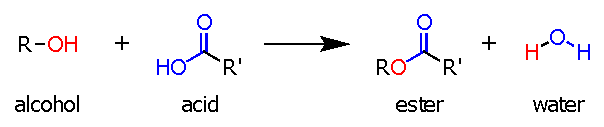
\includegraphics[width=0.7\textwidth]{\figpath/model1_ester-general.pdf}}
	
	One example of a polymerization reaction using this chemistry is the synthesis of poly(6-hydroxycaproic acid) from 6-hydroxycaproic acid monomers:
	
	\centerline{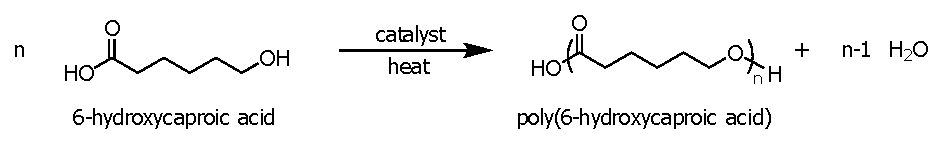
\includegraphics[width=0.9\textwidth]{\figpath/model1_P6HCA.pdf}}

\end{model}


\begin{ctqs}

	\question Consider the 6-hydroxycaproic acid monomer shown in Model \ref{\labelbase:mdl:polyester}: \label{\labelbase:ctq:label-6hcpa}
	
		\begin{enumerate}
			\item As drawn, what type of functional group is on the \emph{left} side of the monomer?
			
				\begin{solution}[1in]
					carboxylic acid (``acid'' is also fine)
				\end{solution}
			
			\item As drawn, what type of functional group is on the \emph{right} side of the monomer?
			
				\begin{solution}[1in]
					alcohol (or hydroxyl)
				\end{solution}
		\end{enumerate}
		
\end{ctqs}

\begin{infobox}

	When a monomer used in a step-growth polymerization has different reactive functional groups on each end, it is called an ``AB-type'' monomer.
	
	When a monomer used in a step-growth polymerization has the same reactive functional group on each end, it is called an ``AA-type'' or ``BB-type'' monomer.

\end{infobox}

\begin{ctqs}
		
		\question Would you classify the poly(6-hydroxycaproic acid) monomer used in this synthesis as an AA-type monomer or an AB-type monomer?  Briefly explain your answer in 1-2 complete sentences.
			
				\begin{solution}[1.75in]
					This is an AB-type monomer, because it has two different reactive functional groups in the same monomer.
				\end{solution}
		
		\question The synthesis of a short 6-hydroxycaproic acid oligomer from three monomers is shown explicitly, below: \label{\labelbase:ctq:6hcpa-oligomer}
	
\vspace{0.25in}	\centerline{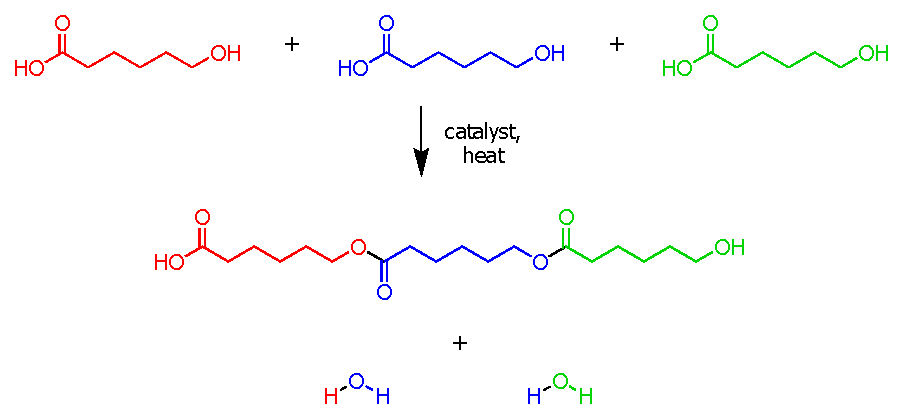
\includegraphics[width=0.9\textwidth]{\figpath/model1_3oligomer-explicit.pdf}}
The molecules are shaded and color-coded so that you can see which atoms in the oligomer came from which monomer.
		
		\begin{enumerate}
		
			\item What type of bonds connect the different monomers in the polymer backbone?
			
				\begin{solution}[1.5in]
					The monomers are connected by ester bonds.
				\end{solution}
		
			\item Explain, in one or two complete sentences, why you think we classify this polymer as a ``polyester'':
			
				\begin{solution}[2in]\instructordisplay{
					We call this polymer a ``polyester'' because it has ester groups in the polymer backbone.
					
					Note: the fact that they are in the backbone is important; if the ester groups are only in the sidechains, the polymer is \emph{not} a polyester - students will address this point in CTQ \ref{\labelbase:ctq:PMA}.
				}\end{solution}
	
			\item When we write the structure of this oligomer as
	
	\centerline{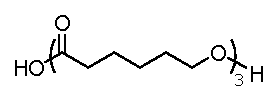
\includegraphics[width=0.25\textwidth]{\figpath/model1_3oligomer-shorthand.pdf}}
	\vspace{-3pt}
	how many different monomer molecules contribute to each repeat unit in the polymer chain?
			
				\begin{solution}[1in]
					one
				\end{solution}
		
			\item Explain, in one or two complete sentences, why we generally abbreviate the product of this reaction as
	
	\centerline{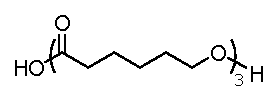
\includegraphics[width=0.25\textwidth]{\figpath/model1_3oligomer-shorthand.pdf}}
	
	rather than as
	
	\centerline{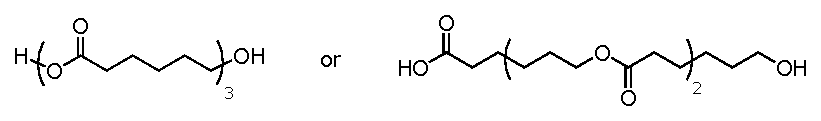
\includegraphics[width=0.7\textwidth]{\figpath/model1_incorrect-shorthand.pdf}}
			
				\begin{solution}[2in]
					We use the first notation because all of the atoms in a single repeat unit come from the same monomer (if you draw these parentheses on the color-coded molecules at the beginning of the question, each pair of parentheses will only have one color of atoms in it).  This is not true for the second and third options.
				\end{solution}
			
		\end{enumerate}
	
	\question Consider the following polymer:\label{\labelbase:ctq:PMA}
	
	\centerline{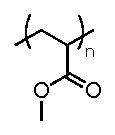
\includegraphics[width=0.1\textwidth]{\figpath/model1_PMA.pdf}}
	
		\begin{enumerate}
				
			\item Does this polymer have ester bonds in the polymer backbone?
			
				\begin{solution}[0.75in]
					No (they are only in the sidechains).
				\end{solution}
		
			\item Would you be able to produce this polymer by esterification reactions of small molecules?  Why or why not?
			
				\begin{solution}[2in]
					No.  This polymer (poly(methyl acrylate)) contains ester bonds, but they are only in the sidechains, not the backbone.  But when we produce a polymer from esterification reactions of small molecules, the ester bonds end up in the polymer backbone.
					
					Put another way, the backbone in this polymer only contains carbon-carbon bonds, which cannot be formed by esterification reactions.
				\end{solution}
			
			\item Based on your answers to the previous two questions, would you classify this polymer as a polyester?  Why or why not?
			
				\begin{solution}[2in]
					No, this is not a polyester because it does not contain ester bonds in the polymer backbone, and cannot be produced by esterification of small molecules.
				\end{solution}
			
		\end{enumerate}
		
\end{ctqs}
	

\clearpage
\begin{model}[Synthesis of a Polyamide]
\label{\labelbase:mdl:polyamide}

Amidation reactions are another type of reaction used to produce polymers by step-growth polymerizations.
For example, acid chlorides can be reacted with primary amines to form an amide bond:
	
	\centerline{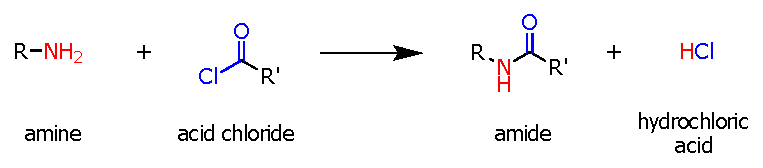
\includegraphics[width=0.7\textwidth]{\figpath/model2_amide-general.pdf}}

Commercially, this reaction is used to produce Nomex, a heat-resistant polymer used in oven mitts and firefighters' protective clothing, among other applications.
A reaction scheme for the synthesis of Nomex is shown below:
	
	\centerline{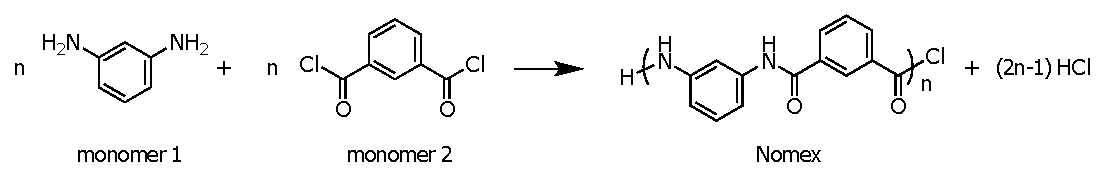
\includegraphics[width=0.9\textwidth]{\figpath/model2_Nomex.pdf}}

\end{model}

\begin{ctqs}
		\question Why is this polymer classified as a polyamide?
			
				\begin{solution}[1.5in]
					This polymer is classified as a polyamide because it has amide bonds in the polymer backbone.
				\end{solution}
		
		\question What functional groups does monomer 1 have?   Would you classify this monomer as an AA-type monomer or an AB-type monomer?
			
				\begin{solution}[0.75in]
					Monomer 1 has two amine groups.  Because it has two of the same reactive group, it is an AA-type monomer.
				\end{solution}
		
		\question What functional groups does monomer 2 have?   Would you classify this monomer as an AA-type monomer or an AB-type monomer?
			
				\begin{solution}[0.75in]
					Monomer 2 has two acid chloride groups.  Because it has two of the same reactive group, it is an AA-type monomer.
				\end{solution}
		
		\question Explain, in one or two complete sentences, why we might describe this reaction as an ``AA+BB''-type polymerization:
			
				\begin{solution}[1.75in]
					This polymer is formed from two AA-type monomers.  Since the two monomers are chemically different, we distinguish them by calling one the ``AA-type'' monomer and the other a ``BB-type'' monomer; thus, we call the polymerization an ``AA+BB''-type polymerization.
					
					This reaction is notably different from the AB-type polymerization in Model 1 because it requires two chemically distinct monomers; in the AB-type polymerization in Model 1, we only needed one type of monomer.
				\end{solution}
		
		\question How many monomers make up each repeat unit?
			
				\begin{solution}[1in]
					two
				\end{solution}
		
		\question A very similar reaction can be used to make Kevlar, the high-strength polymer used in bulletproof vests and cut-resistant gloves.  Given that Kevlar is produced from the following two monomers,
		
	
	\centerline{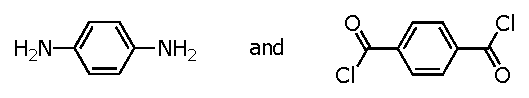
\includegraphics[width=0.5\textwidth]{\figpath/model2_Kevlar-monomers.pdf}}
		
		predict the structure of the Kevlar polymer:
			
				\begin{solution}[2.5in]
					\instructordisplay{\centerline{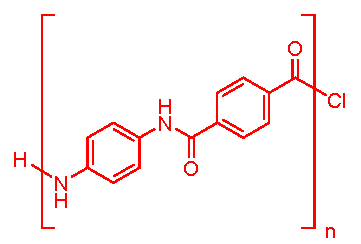
\includegraphics[width=0.4\textwidth]{\figpath/model2_Kevlar.pdf}}
					
					Note: for the purposes of this question, the repeat unit structure is more important than the end groups.  One potential set of end-groups is shown here, although practically speaking, the acid-chloride end group is unlikely to persist - it is very reactive, and would likely hydrolyze to a carboxylic acid.}
				\end{solution}
		
		\clearpage
		\question A similar chemistry can also be used to prepare nylon-6,6, a polymer used in many consumer goods.
		The structure of nylon-6,6 is shown below:
		
			\centerline{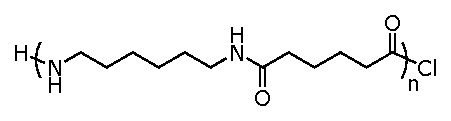
\includegraphics[width=0.45\textwidth]{\figpath/model2_nylon66.pdf}}
			
		What two monomers would you need to combine to make this polymer?
			
				\begin{solution}[2in]
					\instructordisplay{\centerline{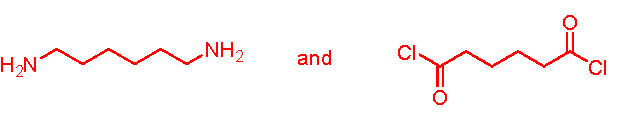
\includegraphics[width=0.6\textwidth]{\figpath/model2_nylon66-monomers.pdf}}}
				\end{solution}
			
\end{ctqs}
	
\begin{infobox}

A polymerization reaction is called a \emph{condensation} polymerization if the reaction produces a small-molecule byproduct that is not part of the polymer chain.

\end{infobox}
	
\begin{ctqs}
		\question Is the esterification reaction in Model \ref{\labelbase:mdl:polyester} a condensation polymerization?  If so, what is the small-molecule byproduct that is produced?
			
				\begin{solution}[1in]\instructordisplay{
					Yes, the reaction in Model \ref{\labelbase:mdl:polyester} is a condensation polymerization. It produces \ce{H2O}.
				}\end{solution}
		
		\question Is the amidation reaction in Model \ref{\labelbase:mdl:polyamide} a condensation polymerization?  If so, what is the small-molecule byproduct that is produced?
			
				\begin{solution}[1in]\instructordisplay{
					Yes, the reaction in Model \ref{\labelbase:mdl:polyamide} is a condensation polymerization. It produces \ce{HCl}.
				}\end{solution}
		
\end{ctqs}

\begin{model}[Other Chemistries used for Step-Growth Polymerization]
\label{\labelbase:model:otherstepgrowthchems}

Shown below are synthetic schemes for a variety of other commercially-important polymers produced by step-growth polymerization:

\vspace{0.1in}

\textbf{a) polycarbonate} (high transparency and impact resistance; used in DVDs, glasses, etc.)
		
			\centerline{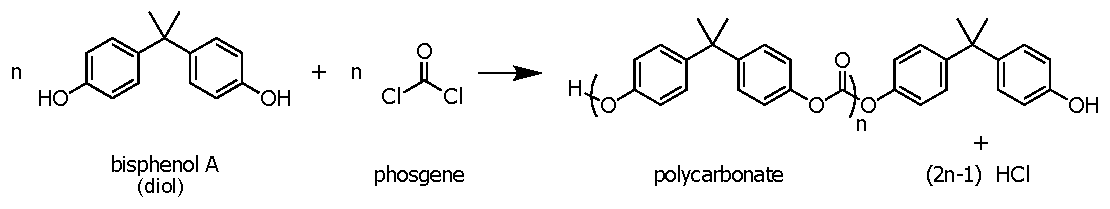
\includegraphics[width=\textwidth]{\figpath/model3_polycarbonate.pdf}}

\vspace{0.1in}

\textbf{b) polyurethanes} (foams; thermoplastic elastomers, e.g. spandex)
		
			\centerline{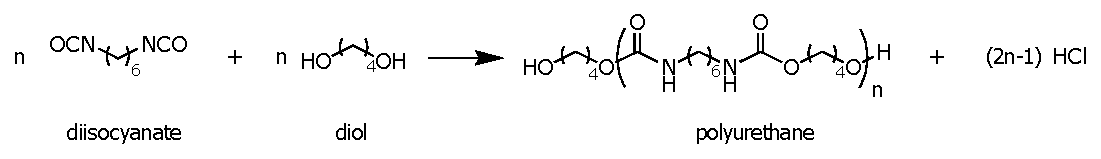
\includegraphics[width=0.9\textwidth]{\figpath/model3_polyurethane.pdf}}

\vspace{0.1in}

\textbf{c) epoxies} (adhesives; coatings)
		
			\centerline{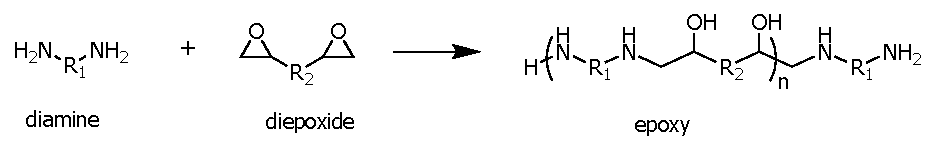
\includegraphics[width=\textwidth]{\figpath/model3_epoxy.pdf}}

\end{model}

\vspace{0.25in}
\begin{ctqs}

		\question Classify each of the reactions in the above Model as either an ``AB-type'' or ``AA+BB-type'' polymerization:
		
			\begin{enumerate}
				\item ~ \begin{solution}[0.6in]AA+BB-type\end{solution}
				\item ~ \begin{solution}[0.6in]AA+BB-type\end{solution}
				\item ~ \begin{solution}[0.6in]AA+BB-type\end{solution}
			\end{enumerate}
			
		% may need another question in here
		
		\clearpage
		\question Complete the following table for the polymerizations depicted in Models 1-3:
		
			\begin{center}
				\begin{tabular}{|c|c|c|c|c|}
				\hline
					Polymer & ``A'' reactive group & ``B'' reactive group & ``ab'' bond formed & \begin{tabular}{c}Small\\ Molecule\\Byproduct\end{tabular} \\\hline
					Polyester &						
						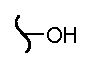
\includegraphics[width=0.12\textwidth]{\figpath/model3_hydroxyl.pdf} &
						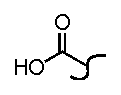
\includegraphics[width=0.15\textwidth]{\figpath/model3_acid.pdf} &
						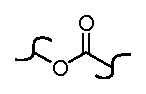
\includegraphics[width=0.15\textwidth]{\figpath/model3_ester.pdf}&
						\answer{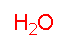
\includegraphics[width=0.08\textwidth]{\figpath/model3_H2O-red.pdf}}\\\hline
					Polyamide &
						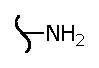
\includegraphics[width=0.12\textwidth]{\figpath/model3_amine.pdf} &
						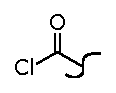
\includegraphics[width=0.15\textwidth]{\figpath/model3_acidchloride.pdf} &
						\answer{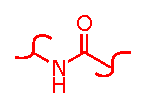
\includegraphics[width=0.15\textwidth]{\figpath/model3_amide-red.pdf}}&
						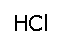
\includegraphics[width=0.08\textwidth]{\figpath/model3_HCl.pdf} \\\hline
					Polycarbonate &
						
\includegraphics[width=0.004\textwidth]{\figpath/model3_blank.pdf}\answer{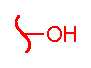
\includegraphics[width=0.12\textwidth]{\figpath/model3_hydroxyl-red-right.pdf}}&
						\answer{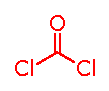
\includegraphics[width=0.15\textwidth]{\figpath/model3_phosgene-red.pdf}}&
						\answer{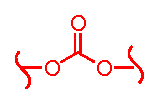
\includegraphics[width=0.15\textwidth]{\figpath/model3_carbonate-red.pdf}}& 
						\answer{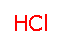
\includegraphics[width=0.08\textwidth]{\figpath/model3_HCl-red.pdf}}\\\hline
					Polyurethane &
						
\includegraphics[width=0.004\textwidth]{\figpath/model3_blank.pdf}\answer{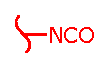
\includegraphics[width=0.12\textwidth]{\figpath/model3_isocyanate-red.pdf}}&
						\answer{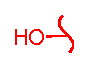
\includegraphics[width=0.12\textwidth]{\figpath/model3_hydroxyl-red-left.pdf}}& 
						\answer{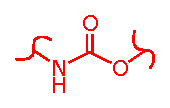
\includegraphics[width=0.15\textwidth]{\figpath/model3_urethane-red.pdf}}&
						\answer{none}\\\hline
					Epoxy &
						
\includegraphics[width=0.004\textwidth]{\figpath/model3_blank.pdf}\answer{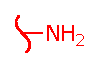
\includegraphics[width=0.12\textwidth]{\figpath/model3_amine-red.pdf}}&
						\answer{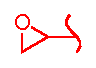
\includegraphics[width=0.12\textwidth]{\figpath/model3_epoxide-red.pdf}}&
						\answer{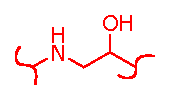
\includegraphics[width=0.15\textwidth]{\figpath/model3_epoxy-red.pdf}}&
						\answer{none} \\\hline
				\end{tabular}
			\end{center}
			
		\vspace{0.25in}
		\question Which of the above polymerization reactions would you classify as condensation polymerizations?  Briefly explain your answer in 1-2 complete sentences.
			
				\begin{solution}[2in]
					The first three reactions (formation of polyesters, polyamides, and polycarbonates) form small-molecule byproducts, so are condensation polymerizations.
					
					The last two reactions (formation of polyurethanes and epoxies) do not form small-molecule byproducts, so are not condensation polymerizations.
				\end{solution}
			
\end{ctqs}
	

\clearpage
\begin{exercises}

		%\exercise (alternate esterification and amidation chemistries? see H&L Tables 2.3 and 2.4)
		
		\exercise \label{\labelbase:exc:AABBester} Although the polymers formed by AB-type and AA+BB-type step-growth polymerizations are similar, there are some subtle but important differences.
			Consider the synthesis of a polyester from the following two monomers:
			
			\centerline{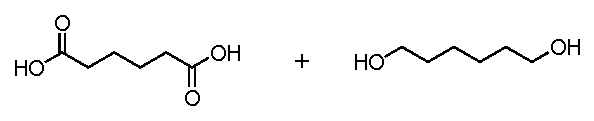
\includegraphics[width=0.6\textwidth]{\figpath/exercises_polyester-AABB-monomers.pdf}}	
			
			\begin{enumerate}
				\item Draw the structure of the polymer that would be formed from this pair of monomers.
					
					\begin{solution}\instructordisplay{
						\centerline{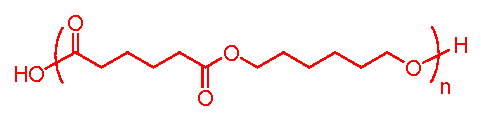
\includegraphics[width=0.4\textwidth]{\figpath/exercises_polyester-AABB-shorthand.pdf}}
					}\end{solution}
					
				\item Compare this structure to the polymer produced from the AB-type monomer in Model \ref{\labelbase:mdl:polyester} (hint: you may find it useful to explicitly draw out a few repeat units).  Are they the same, or different?  If they are different, briefly describe what is different about the two structures.
					
					\begin{solution}\instructordisplay{
						If we explicitly draw out two repeat units of the polymer produced from the AA+BB type monomers, we get something like this:
						
						\centerline{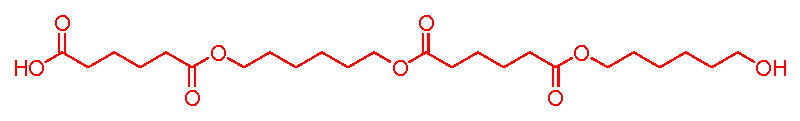
\includegraphics[width=0.7\textwidth]{\figpath/exercises_polyester-AABB-4oligo.pdf}}
						
						On the other hand, if we explicitly draw out the polymer produced from the AB-type monomers, we get
						
						\centerline{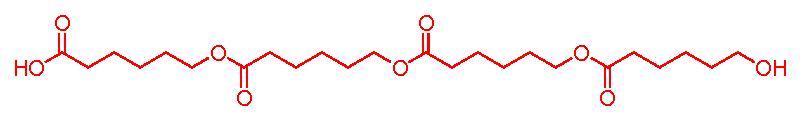
\includegraphics[width=0.7\textwidth]{\figpath/exercises_polyester-AB-4oligo.pdf}}
						
						These structures are very similar; however, as you will notice, the orientation of the ester groups is slightly different: in the polymer produced from AB-type monomers, every ester group is oriented in the same direction, while in the polymer produced from the AA+BB-type monomers, they alternate.
						
						Another consequence is that the effective spacing between carbonyl groups is constant in the polymer produced from AB-type monomers (there are 6 atoms separating each \ce{C=0}), while it varies in the polymer produced from AA+BB-type monomers (where the spacing alternates between 6 and 8 atoms separating each \ce{C=O} group).
						These differences will affect the physical properties of the polymers by changing - among other things - how easy it is for the chains to pack or align with each other.
						
					}\end{solution}
					
			\end{enumerate}
		
		\exercise One of the reasons that polyamides have such useful properties is that the amide groups can form hydrogen bonds between chains, as shown below:
			
			\centerline{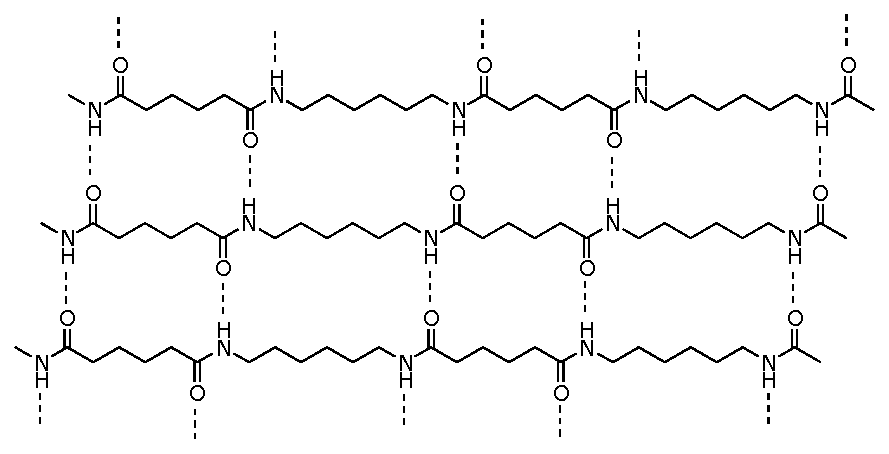
\includegraphics[width=0.7\textwidth]{\figpath/exercises_nylon-network-Hbond.pdf}}	
		
			These inter-chain hydrogen bonds significantly improve the mechanical properties (e.g. stiffness, resilience, etc.) of the material.
			
			Draw an analogous structure for the AA+BB-type polyester that you drew in Exercise \ref{\labelbase:exc:AABBester}.  Can this polymer form inter-chain hydrogen bonds?  Briefly explain your answer, and discuss how you expect the physical properties of the polyester to compare to those of the polyamide.
			
			\begin{solution}\instructordisplay{	
				The analogous structure for the AA+BB-type polyester is
			
			\centerline{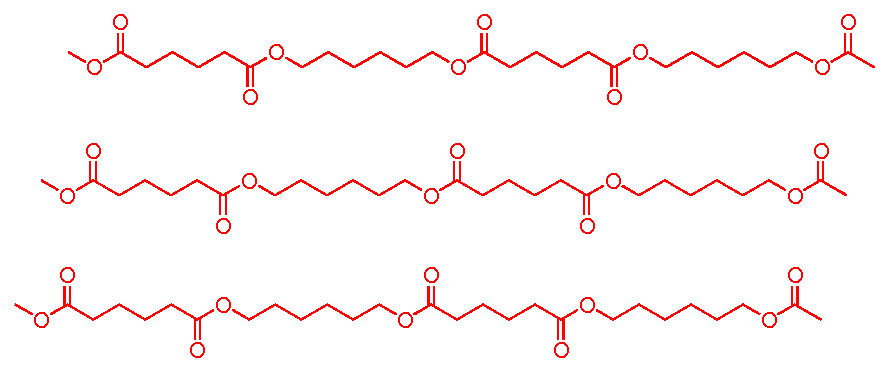
\includegraphics[width=0.8\textwidth]{\figpath/exercises_polyester-network.pdf}}	
			
				While the polyamide was able to form hydrogen bonds because amide \ce{NH} bond (which is polar, and has a partial positive charge on the hydrogen atom which can interact with the partial negative charge on the adjacent chain's carbonyl groups), the polyester lacks this feature - there is no \ce{OH} or \ce{NH} functionality, and it cannot form hydrogen bonds.
				
				Because the polyester does not form inter-chain hydrogen bonds, we should expect it to be much less mechanically stable - it will probably be softer and less robust.
				}\end{solution}
		
		%\exercise (phosgene alternatives for polycarbonate synthesis?)
		
		\exercise The epoxidation reaction shown in Model \ref{\labelbase:model:otherstepgrowthchems} formed a linear polymer with secondary amines.  However, secondary amines can also attack epoxides.  Draw out the polymer structure that you would expect to generate if this occurs.  How would you describe this polymer architecture?
		
			\begin{solution}\instructordisplay{
				If the secondary amines can also attack epoxides, they will generate branched polymers, as shown below:
			
			\centerline{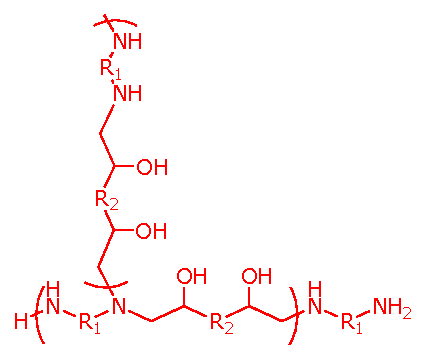
\includegraphics[width=0.4\textwidth]{\figpath/exercises_epoxy-branched.pdf}}	
				
				Note that the polymer chain can keep growing from this branch point, hence the parentheses on the branch as well as the main chain.			
				Eventually, this branch may react with another growing polymer chain, so if this process continues, we will eventually end up with a crosslinked polymer network.
				
				Note that most commercially available epoxy resins use amines with more than two nitrogens, so the monomer is not just a ``BB-type'' monomer, but may be a \ce{B3} or \ce{B4}-type monomer (where the subscript indicates the number of reactive B functional groups, or in this case, the number of amines).
				Similarly, while students were only asked to consider linear polyurethanes in this activity, commercial polyurethane foams typically contain ``polyols'' with 3 or more hydroxyl groups to promote crosslinking.
				
				The formation of networks from multi-functional monomers will be considered in more detail in a later activity.
				
			}\end{solution}
		
\end{exercises}
	
\end{activity}